\scanpage{181}
\mspage{738}

\[
\text{(2)}\qquad
\mathcal L(\Pi)=
\varinjlim_{\substack{\Pi_i\text{ normal}\\
\text{of finite index}\\
\text{in }\Pi}}
\mathcal L_0^{\unsure{\natural|\sharp}}(\Pi_i).
\]

\margin{N.B. If $\Pi_i$ is not normal in
$\Pi$, we can define
$\mathcal L_0^{\unsure{\natural|\sharp}}(\Pi_i)$ as the subset
of $\mathcal L(\Pi_i)$ formed by the loop
structures \inserted{$\lambda$} ``invariant under $\Pi$'', i.e. such that
for $\forall g\in\Pi$, we have that $\lambda$ (on $\Pi_i$) and
$\unsure{\mathrm{int}(g)|\mathrm{Int}(g)}\lambda$
(on $\unsure{\mathrm{int}(g)|\mathrm{Int}(g)}(\Pi_i)$) coincide in
$\Pi_i\cap\unsure{\mathrm{Int}(g)|\mathrm{int}(g)}(\Pi_i)$
(which is of finite index in $\Pi\ldots$)}

\deleted{We say that a}
the canonical morphisms ($\Pi_i$ normal of finite index
in $\Pi$)
\[
\text{(3)}\qquad
\diagram{\begin{tikzcd}
\mathcal L_0^{\unsure{\natural|\sharp}}(\Pi_i) \arrow[r] & \mathcal L(\Pi)
\end{tikzcd}}
\]
are injective. If $\lambda\in\mathcal L(\Pi)$, we say that
$\lambda$ is an \uline{L-structure}\unsure{.} on $\Pi$,
\inserted{$(\Pi,\lambda)$ is called an \uline{L-group},}
(and if
$\lambda\in\operatorname{Im}(\mathcal L_0^{\unsure{\natural|\sharp}}(\Pi_i)\to\mathcal L(\Pi))$),
we say that $\Pi_i$ is
a subgroup of definition of the L-group
$\Pi$ -- we regard it as a
group with loops via the unique $\lambda_i\in\mathcal L_0^{\unsure{\natural|\sharp}}(\Pi_i)$
giving rise to $\lambda$.

Let $\Pi$ be a discrete group, $\unsure{\Pi'_0|\Pi_0}$ a
subgroup of $\Pi$ of finite index. Then
we have a canonical homomorphism
for induction of L-structures
\[
\text{(4)}\qquad
\diagram{\begin{tikzcd}
\unsure{\mathcal L|\mathcal L_0}(\Pi) \arrow[r,hook] & \mathcal L(\Pi')
\end{tikzcd}}
\]
which is injective, and whose image consists
of the set of L-structures on $\Pi'$ that are
\scanpage{182}

``invariant under $\Pi$'' in an obvious sense.
In particular, if we have an \uline{extension}
of a finite group \inserted{$G$} by a
discrete group $\Pi_0$, then the $L$ structures on
$\Pi$ correspond to the $L$-structures
on $\Pi_0$ invariant under
$\Pi/\Pi_0\deleted{\unsure{\simeq G}}\inserted{\longrightarrow\unsure{\mathrm{Autext}}(\Pi_0)}$,
operating on the \unsure{set} of $L$-structures of $\Pi$
in an obvious way. [\uline{N.B.} $\Pi\mapsto\mathcal{L}(\Pi)$ is
a functor in the \uline{outer groups}
$\Pi$, with \uline{outer isomorphisms}
as arrows $\ldots$ ]

Standard example: let $X$ be an
anabelian surface ``of finite character'' \inserted{\unsure{0-connected}},
$G$ a finite group operating on $X$,
\[
\tag{\deleted{\unsure{4}}\inserted{5}}
\Pi=\Pi_1(X,G;\bullet)
\]
where $a$ is a base point of $X$, so
that we have an exact sequence
\[
\tag{6}
\diagram{\begin{tikzcd}[column sep=large,row sep=small]
1 \arrow[r,no head] & \Pi_0 \arrow[r] \arrow[d,equal] & \Pi \arrow[r] & G \arrow[r,no head] & 1 . \\
& \Pi_1(X,\bullet) & & &
\end{tikzcd}}
\]
We then have on $\Pi_0$ a loop structure
\scanpage{183}
\mspage{739}

invariant under the outer operations of $G$, hence
an $L$-structure on $\Pi$. It seems
that $\forall$ $L$-group is isomorphic to
a group obtained this way --- but this is
a result that seems
deep (essential\textsuperscript{ly} equivalent to that \unsure{of|of the}
\inserted{the existence} \inserted{of}
fixed points of finite subgroups of
Teichmüller groups $\ldots$), and which is
not completely understood. We should
\inserted{bring out} a general ``good statement'', linking the
$2$-category of $L$-groups, with that of
surfaces \inserted{$X$ of finite character, \deleted{\unsure{by some}}}
equipped \unsure{with a|with a} ``\unsure{signature}'' \inserted{$\underline{d}$} with
finite\deleted{\unsure{e}} support (with values in $\mathbb{N}^{*}$)
\inserted{punctured}, by associating to
such a surface its $\Pi_1(X,\underline{d},a)$,
relative to a point \deleted{base} $a\in X-\operatorname{supp}\underline{d}$.
Excluding a few singular cases \inserted{``trivial''}, we
should then find an $L$-group $\Pi$,
isomorphic to a $\Pi_1(X;G,a)$\unsure{,|;} with $G$
operating \uline{faithfully}, which \inserted{should} be expressed
\scanpage{184}

in terms of $\Pi$ by the fact that
the centralizer of $\forall$ subgroup
of finite index in $\Pi$ is reduced to $\{e\}$.
\unsure{This|This} should give a complete
\inserted{intrinsic} description, in topological terms, of the
$L$-groups having this additional property.
There would then still be
some work of \unsure{fitting together} to do,
in terms of certain extensions of
such $L$-groups by finite groups,
to \unsure{treat|find} the general case.
Moreover, we should make the connection
with the associated ``$L$-Galois topoi'',
paraphrasing the corresponding
developments on Galois topoi etc.
associated to groups with loops.
\scanpage{185}
\mspage{740}

It could be that the ``right'' general context
for defining and studying general
Teichmüller groups is that
of $L$-groups, rather than that of
groups with loops.

Taking for example the group \deleted{$\unsure{\mathfrak{M}|\mathfrak{S}}$}
\[
\tag{4}
\begin{aligned}
\deleted{\unsure{\mathfrak{M}_{0,3}^{+}|\mathfrak{S}_{0,3}^{+}}}\mathfrak{S}_{0,3}^{+}
&\simeq \mathrm{Sl}(2,\mathbb{Z})/\{\pm1\}\\
&\simeq \Pi_1(U_{0,3}(\mathbb{C}),\mathfrak{S}_3;-\overline{j}),
\end{aligned}
\]
this is equipped with an $L$-structure,
which can be defined in terms of
the unique conjugacy class of the
subgroup \inserted{$L_0$} generated by
$\varepsilon_0=\begin{pmatrix}1&-1\\0&1\end{pmatrix}$,
or of $L_1$ generated by
$\varepsilon_1=\begin{pmatrix}1&0\\1&1\end{pmatrix}$.
The $L$-group \inserted{(\uuline{discrete})} has the remarkable
property that every \inserted{$L$-}automorphism
\inserted{``direct'' (inducing the identity on the \unsure{orientation} module)}
of it is inner. It could
be that this property, added to
the property that the center is trivial (or
better, perhaps, that the centralizer
\scanpage{186}

of every subgroup of finite index is
reduced to $\{1\}$) characterizes $\mathfrak{S}_{0,3}^{+}$ up to
(nonunique) isomorphism.

N.B. To prove that every direct \inserted{$L$-}\unsure{automorphism|automorphism}
\inserted{$u$} of $\deleted{\unsure{\mathfrak M}}\mathfrak{S}_{0,3}^{+}$ is inner, the
essential point seems to me to be to prove
that $u$ preserves the subgroup
$\Pi_{0,3}$, kernel of
\[
\diagram{\begin{tikzcd}[column sep=large]
1 \arrow[r] & \Pi_{0,3} \arrow[r] & \deleted{\unsure{\mathfrak M}}\mathfrak{S}_{0,3}^{+} \arrow[r] & \mathfrak{S}_3 \arrow[r] & 1 .
\end{tikzcd}}
\]

In fact, every automorphism of
the group structure of $\mathfrak{S}_{0,3}^{+}$
(not necessarily an $L$-\unsure{automorphism|automorphism})
preserves the normal subgroup
$\Pi_{0,3}$. This follows from the

\uline{Lemma} Let \inserted{$\Pi\subset\mathfrak{S}_{0,3}^{+}$}
be a normal subgroup such
that $\mathfrak{S}_{0,3}^{+}/\Pi\simeq\mathfrak{S}_3$, then $\Pi=\Pi_{0,3}$.
More precisely, every surjective homomorphism
$p:\mathfrak{S}_{0,3}^{+}\deleted{\unsure{\Pi}}\longrightarrow\mathfrak{S}_3$ is conjugate to the canonical
homomorphism (hence its kernel is $\Pi_{0,3}$).

\uline{Proof} \deleted{Consider a surjective homomorphism}
\inserted{We use the presentation}
of $\mathfrak{S}_{0,3}^{+}$ by $\rho^3=\sigma^2=1$,
\scanpage{187}
\mspage{741}

which implies that a homomorphism $p$ from $\mathfrak S_{0,3}^{+}$ to another group, whose image is not of order $1,2$ or $3$ i.e. of order $\geq 4$, sends $\rho$ and $\sigma$ resp. to elements of order $3$ and of order $2$. So if the image is $\mathfrak S_3$, $\rho$ is sent to $\dot\rho$ or $\dot\rho^{-1}$ (we may suppose, conjugating if necessary \inserted{by $\dot\sigma_\infty$,} that it is $\dot\rho$) and $\sigma$ is sent to $\deleted{\unsure{\dot\sigma}}\;\dot\sigma_0,\dot\sigma_1$ or $\dot\sigma_\infty$ (we may suppose, conjugating by $\dot\rho$ or $\dot\rho^2$ if necessary, that it is $\dot\sigma_\infty$), and we win.

We may call the \uline{Teichmüller group} of an L-group $\Pi$, the group of its outer L-automorphisms --- or perhaps, better, the group of outer L-automorphisms of the subgroup $\Pi^+$ (of index $1$ or $2$) of $\Pi$, consisting of the $g\in\Pi$ such that the automorphism $\operatorname{int}(g)$ is direct. The property envisaged for $\mathfrak S_{0,3}^{+}$ is that its ``direct'' Teichmüller group is reduced to $1$. The property

\scanpage{188}

corresponding to this for the \inserted{L-}group $\mathfrak S_{0,3}\simeq\mathrm{Gl}(2,\mathbb Z)/\pm1$ is that every \deleted{group} \inserted{L-}automorphism of the subgroup $\mathfrak S_{0,3}^{+}$ is induced by a unique element of $\mathfrak S_{0,3}$. This property is perhaps characteristic of the \uline{discrete} L-group $\mathfrak S_{0,3}$.

\figure{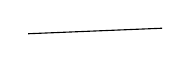
\begin{tikzpicture}
\draw (0,0) -- (1.7,0.07);
\end{tikzpicture}}

I feel like presenting in a slightly different form the notion of L-group\inserted{ $\Pi$,} in terms of the datum of a $\mathbb Z$-module $T$ free of rank $1$ (the $\mathbb Z$-module of orientations) and of a\deleted{\unsure{e}} \deleted{family} \inserted{finite set} $(k_i^{\unsure{\natural|\sharp}})_{i\in I}$ of \uline{germs} \uline{of homomorphisms} that are outer
\[
\begin{gathered}
k_i^{\unsure{\natural|\sharp}}:\quad \deleted{\unsure{\mathbb Z}}\inserted{T}\longrightarrow\Pi
\qquad (i\in I)\\
(\text{\uline{germ} of outer homomorphism})
\end{gathered}
\tag{5}
\]
,

where the notion of ``germ'' is relative to that of subgroups of finite index of $T$. \deleted{The axiom to put in is} \inserted{\unsure{For} such a datum,}

\scanpage{189}
\mspage{742}

and any subgroup \deleted{\unsure{to}} $\Pi_0$ of $\Pi$ of finite index, we find \inserted{for $\forall i$} a set of germs of outer homomorphisms
\[
T\longrightarrow\Pi_0
\]
induced by the actual homomorphisms \deleted{\unsure{outer}} $nT\longrightarrow\Pi$ of the class $k_i^{\unsure{\natural|\sharp}}$ --- we find a finite number of germs of outer homomorphisms $T\longrightarrow\Pi_0$ for fixed $i$, hence also for $i$ varying in $I$. This said, the only axiom of an L-structure, it is that we can find a subgroup $\Pi_0$ of finite index, such that the ``induced structure'' comes from a loop structure on $\Pi_0$.

We can generalize the notion of L-structure, taking inspiration from the preceding definition (for example), and dropping the requirement there that $\Pi_0$ be of finite index --- but while

\scanpage{190}

taking care on the other hand that $\Pi_0$ be \uline{normal}. We require that \deleted{the} for $\forall i\in I$, the germs of homomorphisms $k_i:\deleted{\unsure{n}}T\longrightarrow\Pi$ of the class $k_i^{\unsure{\natural|\sharp}}$ factor through $\Pi_0$ --- which gives a set of \inserted{germs of }outer homomorphisms from $T$ to $\Pi_0$ ---
\margin{N.B. it is not clear a priori that this set of germs of outer homomorphisms is finite}
and we require that this \deleted{set of} \inserted{structure in question} on $\Pi_0$ come \inserted{(for suitable $\Pi_0$)} from a loop structure on $\Pi_0$, \unsure{$\xi$|\&} obviously uniquely determined, once $\Pi_0$ has been chosen. As for $\Pi_0$, it is defined up to commensurability --- i.e. if $\Pi_0,\Pi'_0$ will do, then $\Pi_0\inserted{\cap}\Pi'_0$ is of finite index in $\Pi_0$ and $\Pi'_0$, and will do as well.

\deleted{Taking inspiration from the ``metabelian'' terminology,} I feel like (for want of a better suggestion) calling the groups $\Pi$ equipped with such a